\documentclass[style=njit,orient=landscape]{powerdot}
\pdsetup{
  palette=njit,
  logohook=tl,
  logopos={0.005\slidewidth,0.995\slideheight},
  logocmd={
\includegraphics[trim=0 -1 0 0,clip,width=.2\slidewidth,height=.09\slideheight]{njit.eps}},
  lf={\color{black}Overleaf - \LaTeX{} Documents},
  %lf={\color{black}\sectiontitle},
  cf={\color{black}},
  theslide={\color{black}\arabic{slide}~/~\pageref*{lastslide}}
}
%\definecolor{pdcolor2}{RGB}{241,231,200}%lucream
%\definecolor{pdcolor3}{RGB}{102,55,0}%lubrown
\definecolor{lucyan}{RGB}{0,164,228}
\definecolor{lumagenta}{RGB}{236,81,157}
\definecolor{lugold}{RGB}{255,196,35}
\definecolor{lupurple}{RGB}{125,129,190}

\usepackage{mathtools,amsthm,amssymb,amsfonts}
\usepackage{pifont,tgpagella,marvosym,wasysym}
\usepackage{multicol,multirow}
\usepackage{fancyvrb,listings}
\usepackage{showexpl,enumitem}
\usepackage{graphicx}
\usepackage{rotating}

\renewcommand{\descriptionlabel}[1]%
   {\color{pdcolor2}\textbf{#1}}
\newcommand{\cmark}{\ding{51}}

\lstset{
  language={[LaTeX]TeX},
  %alsolanguage={PGF/TikZ},
  frame=single,
  framesep=\fboxsep,
  framerule=2pt,
%  frameshape={RYRYNYYYY}{yny}{yny}{RYRYNYYYY},
%  fillcolor=\color{pdcolor2},
  rulecolor=\color{pdcolor2},
  xleftmargin=\dimexpr\fboxsep+\fboxrule,
  xrightmargin=\dimexpr\fboxsep+\fboxrule,
  breaklines=true,
  basicstyle=\scriptsize\tt,
  keywordstyle=\color{cyan}\sf,
  morekeywords={part,chapter,subsection,subsubsection,paragraph,subparagraph},
  identifierstyle=\color{magenta},
  commentstyle=\color{pdcolor3},
  backgroundcolor=\color{pdcolor2!30!black},
  tabsize=2,
  columns=flexible,
  escapeinside={\%*}{*)},
}
\usepackage[utf8]{inputenc}

\title{Overleaf for Writing \LaTeX{} Documents}
\author{Jill Lagerstrom \and Alex Pacheco}
\date{September 19, 2024}

\begin{document}

\maketitle
\begin{wideslide}[toc=,bm=]{Overview}
  \tableofcontents[content=sections]
\end{wideslide}
\scriptsize

\section[slide=false]{\TeX{} \& \LaTeX{}}
%\begin{wideslide}[toc=,bm=]{Overview}
%  \tableofcontents[content=currentsection,type=0]
%\end{wideslide}
%	\section[tocsection=true,slide=true]{Introduction}
\begin{slide}[bm={What is \TeX{} \& \LaTeX?}]{What is \TeX{}?}
  \begin{itemize}
  \item \TeX{} is a low-level markup and programming language created by Donald Knuth to typeset documents attractively and consistently.
  \item \TeX{} is a programming language in the sense that it supports the if-else construct: you can make calculations with it (that are performed while compiling the document), etc., but you would find it very hard to do anything else but typesetting with it.
  \item The fine control \TeX{} offers over document structure and formatting makes it a powerful and formidable tool.
  \item \TeX{} is renowned for being extremely stable, for running on many different kinds of computers, and for being virtually bug free.
  \item \TeX\, is a popular means by which to typeset complex mathematical formulae; it has been noted as one of the most sophisticated digital typographical systems in the world.
  \item Programming in \TeX{} generally progresses along a very gradual learning curve, requiring a significant investment of time to build custom macros for text formatting.
  \item Document preparation systems based on \TeX{}, consisting of collections of pre-built macros, exist making it easier for the user to create documents without the need to learn the \TeX{} language.
  \end{itemize}
\end{slide}	

\begin{slide}[bm={What is \LaTeX{}?}]{What is \LaTeX{}?}
  \begin{itemize}
  \item \LaTeX{} is a macro package based on \TeX{} created by Leslie Lamport.
  \item Its purpose is to simplify \TeX{} typesetting, especially for documents containing mathematical formulae.
  \item Popular in academia, especially in mathematics, computer science, economics, engineering, physics, statistics, and quantitative psychology.
  \item Many of the academic publishing houses such as American Institute of Physics, Elsevier, etc provide templates to prepare manuscripts in \LaTeX{}.
  \item Since \LaTeX{} comprises a group of \TeX{} commands, \LaTeX{} document processing is essentially programming.
  \item Using \LaTeX{} to create documents is a WYSIWYM (What You See Is What You Mean) approach rather than 
  \item[] WYSIWYG (What You See Is What You Get) approach of Microsoft Word and Libre Office.
  \item In \LaTeX{}, you create a text file in \LaTeX{} markup, which then needs to be compiled to produce the final document, most commonly is postscript (ps) or portable document format (pdf).
  \item The final document can be viewed uniformly on any Operating System using any version of the document viewer.
  \end{itemize}
\end{slide}

\begin{slide}[bm={Advantages of \LaTeX{}?}]{Advantages of \LaTeX{}?}
  \begin{itemize}
  \item Document sources can be read with any text editor.
  \item You can concentrate purely on the structure and contents of the document, not get caught up with superficial layout issues.
  \item You don't need to manually adjust fonts, text sizes, line heights, or text flow for readability, as \LaTeX{} takes care of them automatically.
  \item In \LaTeX{} the document structure is visible to the user, and can be easily copied to another document.
  \item The layout, fonts, tables and so on are consistent throughout the document.
  \item Mathematical formulae can be easily typeset.
  \item Indexes, footnotes, citations and references are generated easily.
  \item Since the document source is plain text, tables, figures, equations, etc. can be generated programmatically with any language.
  \item You are forced to structure your documents correctly.
  \end{itemize}
\end{slide}

\begin{slide}[bm={Disadvantages of \LaTeX{}?}]{Disadvantages of \LaTeX{}?}
  \begin{itemize}
  \item \LaTeX{} is WYSIWYM and not WYSIWYG approach
  \item[] i.e. you can't see what the final version will look like while typing.
  \item You need to know the necessary commands for the markup language.
  \item[] i.e. there is no drop-down menu to create the document content such as equations, tables, inserting figures etc, you need to know how to enter those in a text editor.
  \item It can sometimes be difficult to obtain a certain look for the document.
  \end{itemize}
\end{slide}

\section[slide=false]{Overleaf}
%\begin{wideslide}[toc=,bm=]{Overview}
%  \tableofcontents[content=currentsection,type=0]
%\end{wideslide}
\begin{slide}{What is Overleaf?}
 \begin{itemize}
  \item an online collaborative writing and publishing tool that makes the whole process of writing, editing and publishing scientific documents much quicker and easier. 
  \item provides the convenience of an easy-to-use \LaTeX{} editor with real-time collaboration and the fully compiled output produced automatically in the background as you type.
  \item makes the journal submission process smoother for \LaTeX{} users across many academic publishers.
 \end{itemize}
\end{slide}

\begin{slide}{Why use Overleaf?}
\begin{itemize}
    \item cloud based product that only needs a web browser.
    \item effortless sharing with collaborators.
    \item compiles your project in the background, so you can see the output PDF right away.
    \item real-time commenting and integrated chat, you can discuss your work without having to switch to email, printed versions or any other tool. 
    \item Rich Text and \LaTeX{} modes if you prefer to see less of the code when you’re writing
    \item Overleaf shows you errors and warnings as you go, so you can catch them early, and it shows them inline, so you don't have to find them in the \LaTeX{} log.
    \item Write your thesis, create a calendar, make amazing presentations with the beamer package and create posters to showcase your work, all from a wide selection of popular templates. 
    \item The real-time preview also helps when you're working with complicated tables, tikz figures and pgfplots graphs.
\end{itemize}
\end{slide}

\begin{slide}{Lehigh's Overleaf Commons Subscription}
\begin{itemize}
    \item Overleaf Professional accounts – for students, faculty and staff.
    \begin{itemize}
        \item Unlimited collaborators 
        \item Full document history
        \item Reference Manager Sync
        \item Dropbox and Git/Github integration
        \item 20GB of storage
    \end{itemize}
    \item Hassle-free license management – users simply register with their institutional email address on Overleaf (or add it to their existing Overleaf account) to join your Overleaf Commons license and receive their upgrade automatically.
\end{itemize}
\end{slide}

\section[slide=false]{Getting Started}

\begin{slide}{How do I Sign Up}
\begin{itemize}
    \item Visit \url{https://www.overleaf.com/register}
    \item Sign up with your email address, Google or ORCID.
    \begin{itemize}
        \item Your NJIT email address and Google account is valid as long as you are a student, staff or faculty.
        \item Your Overleaf account is tied to the registered email address. If your email address is deactivated, you lose access to your overleaf account.
        \item Consider using your personal email or Google account for registration.
        \item Go to Account Settings and add your NJIT email as your secondary email to convert to a Pro account.
    \end{itemize}
\end{itemize}
\end{slide}

\begin{slide}{How do I Create a document}
    \begin{itemize}
        \item Click on New Project in the left sidebar.
        \item Choose from 
        \begin{description}
            \item[Blank Project]: Start with a empty .tex file.
            \item[Example Project]: Start with an example article that overleaf provides.
            \item[Upload Project]: Upload a zip file containing an existing \LaTeX{} project i.e. at least one .tex file.
            \item[Import from Github]: Import an existing \LaTeX{} project from your Github account.
        \end{description}
    \end{itemize}
\end{slide}

\begin{slide}[method=direct]{My First \LaTeX{} Document}
\begin{itemize}
    \item Start with a Blank Document and add the following lines to it \begin{lstlisting}
\documentclass[10pt]{article}

\title{My First Document}
\author{Enter your name}
\date{\today}

\begin{document}

\maketitle
\tableofcontents

\section{My First Section}\label{section1}
Hello World!

\section{My Second Section}
In Sec. \ref{section1}, we said Hello to the World.

\end{document}
\end{lstlisting}
    \item Watch the document compile on the right window. Click "Recompile" for compiling the document on demand. 
\end{itemize}
\end{slide}



\section[slide=false]{Document Structure}
%\begin{wideslide}[toc=,bm=]{Overview}
%  \tableofcontents[content=currentsection,type=0]
%\end{wideslide}

\begin{wideslide}[toc=,method=direct]{\LaTeX{} File Structure}
  \begin{itemize}
  \item When \LaTeX{} processes an input file, it expects it to follow a certain structure.
  \item Every \LaTeX{} input file must contain the commands,
    \begin{lstlisting}
\documentclass{...}

\begin{document}
...
\end{document}
    \end{lstlisting}
  \item The area between \lstinline|\documentclass{...}| and \lstinline|\begin{document}| is called the {\bf Preamble}.
  \item The document content goes between the \lstinline|\begin{document}| and \lstinline|\end{document}| commands,
    \begin{lstlisting}
\begin{document}
   ...
\end{document}
    \end{lstlisting}
%  \item The reason for marking off the beginning of your text is that \LaTeX{} allows you to insert extra setup specifications before it.
%  \item The reason for marking off the end of your text is to provide a place for \LaTeX{} to be programmed to do extra stuff automatically at the end of the document, like making an index.
  \end{itemize}
\end{wideslide}

\begin{wideslide}{Preamble}
  \begin{itemize}
  \item The Preamble is anything that comes before the main document.
  \item It is used for
    \begin{itemize}
    \item Defining the type of document.
    \item Defining the top matter i.e. title, author, etc.
    \item Applying global formatting including changing page layout from the default.
    \item Including packages to add functionality.
    \end{itemize}
  \end{itemize}
\end{wideslide}

\begin{wideslide}[bm={Document Types},method=direct]{Document Types}
  \begin{itemize}
  \item The first uncommented line of the \LaTeX{} document needs to describe the type of document that you are creating using
  \item[] \lstinline|\documentclass[options]{documenttype}|
  \item \LaTeX{} can be used to create documents of various types
    \begin{enumerate}
    \item article
    \item report
    \item book
    \item letter
    \item beamer\footnote{\tiny For Tutorial, visit \url{http://www.hpc.lsu.edu/training/archive/tutorial.php}}, {\color{pdcolor2}powerdot}\footnote{\tiny{\sc this presentation}, style file included in downloads}, {\color{red}prosper or seminar\footnote{\tiny Not popular anymore, use beamer or powerdot}} for Presentations
    \end{enumerate}
  \item The difference between article, report and book is in the document structure and presentation:
  \item In article type, there is no chapter and the title page and document content can appear on the first page.
  \item In report and book, the title page is the first page and document content begins on the second page onwards.
  \item In article and report, there is an abstract environment to write the abstract of the article or report that you are writing.
  \vspace{0.2cm}
  \end{itemize}
\end{wideslide}

\begin{wideslide}[bm={documentclass options}]{documentclass options}
  \begin{itemize}[][itemsep=1pt,parsep=1pt]
  \item The options to documentclass are used to define a predetermined structure for the document.
  \item The most commonly used options are defining
    \begin{itemize}[][itemsep=1pt,parsep=1pt]
    \item font size: 10pt (default), 11pt or 12pt
    \item paper size: letterpaper (default), legalpaper, executivepaper, a4paper, a5paper or b5paper
    \item orientation: portrait (default) or landscape
    \item page format: onecolumn (default) or twocolumn
    \end{itemize}
  \item Options that depend on document type
    \begin{itemize}[][itemsep=1pt,parsep=1pt]
    \item Where to print page numbers for book, report and article
      \begin{itemize}[][itemsep=1pt,parsep=1pt]
      \item[{\bfseries\color{pdcolor2}oneside}] page numbers are printed the same on even and odd pages, default for article \& report
      \item[{\bfseries\color{pdcolor2}twoside}] page number appears on the right side for odd pages and on the left for even pages, default for book
      \end{itemize}
    \item Where new chapters begin in the book and report class
      \begin{itemize}[][itemsep=1pt,parsep=1pt]
      \item[{\bfseries\color{pdcolor2}openright}] chapters start on the right hand insert blank page if necessary i.e. odd numbered page
      \item[{\bfseries\color{pdcolor2}openany}] chapters always start on the next page
      \end{itemize}
    \item Where the title appears
      \begin{itemize}[][itemsep=1pt,parsep=1pt]
      \item In book and report classes, the title appears on the first page separate from the document content
      \item In article class, the title appears on the first page followed by the document content
      \item Use {\bfseries\color{pdcolor2}titlepage} and {\bfseries\color{pdcolor2}notitlepage} to override this standard behavior.
      \end{itemize}
    \end{itemize}
  \end{itemize}
\end{wideslide}

\begin{wideslide}[toc=,bm=,method=direct]{documentclass options}
  \begin{itemize}
    \item Other options commonly used
      \begin{description}
        \item[{leqno}]: display equation numbers on the left rather than the default right
        \item[{fleqn}]: displayed formulas are flushed left instead of default centered
        \item[{draft}]: mark lines that are too wide with a thick black bar
        \item[{final}]: default, do not mark lines that are too wide.
      \end{description}
    \item Add some options to documentclass to create your second document.
  \end{itemize}
  \begin{lstlisting}
\documentclass[12pt,twocolumn,fleqn]{article}
  \end{lstlisting}
\end{wideslide}

\begin{wideslide}[method=direct]{Creating a Title Page}
  \begin{itemize}[][itemsep=1pt,parsep=1pt]
  \item To create a title page \LaTeX{} has three commands.
    \begin{itemize}[][itemsep=1pt,parsep=1pt]
      \item \lstinline|\title{Title}| where Title is the title of your article, book or report.
      \item \lstinline|\author{FirstName LastName}|, if there are multiple authors, list them all delimited by a comma (,) or and.
      \item \lstinline|\date{\today}| to set the date when the article was created i.e. today
      \item[] If the date required is different from today, add the date that you need as in \lstinline|\date{Feb. 29, 2016}|
    \end{itemize}
    \item If you are publishing a journal article, please see their \LaTeX{} templates and style files. Most of their style and class files  define additional commands such as \lstinline|\affiliation{...}|, \lstinline|\institution{...}|, etc.
    \item To create the actual page, you need to add \lstinline|\maketitle| in your document i.e. after the \lstinline|\begin{document}| command.
    \item The \lstinline|\maketitle| is almost always the first line of your document content.
  \end{itemize}
      \begin{lstlisting}
\documentclass[12pt,twocolumn,fleqn]{article}
\title{Simple \LaTeX{} Document}
\author{Alex Pacheco, Bhupender Thakur, Feng Chen and Le Yan}
\date{\today}
\begin{document}
\maketitle
\end{document}
      \end{lstlisting}
\end{wideslide}

\begin{wideslide}[bm={Document Structure},method=direct]{Structuring a \LaTeX{} Document}
  \begin{itemize}
    %  \item A \LaTeX{} document consists of two parts
    %    \begin{enumerate}
    %    \item Preamble
    %    \item Main Document
    %      \begin{itemize}
  \item Document Content i.e. everything between the \lstinline|\begin{document}| and \lstinline|\end{document}| is partitioned into
  \end{itemize}
  \begin{center}
    \begin{tabular}{llcl}
      \hline
      Section & Command & Level & Comment\\
      \hline
      part & \lstinline|\part{title}| & -1 & not in letters \\
      chapter & \lstinline|\chapter{title}| & 0 & only in book and report \\
      section & \lstinline|\section{title}| & 1 & not in letters \\
      subsection & \lstinline|\subsection{title}| & 2 & not in letters \\
      subsubsection & \lstinline|\subsubsection{title}| & 3 & not in letters \\
      paragraph & \lstinline|\paragraph{title (optional)}| & 4 & not in letters \\
      subparagraph & \lstinline|\subparagraph{title (optional)}| & 5 & not in letters \\
      \hline
    \end{tabular}
  \end{center}
  %    \begin{itemize}
  %    \item abstract (article and report only)
  %    \item part (-1)
  %    \item chapter (0)
  %    \item section (1)
  %    \item subsection (2)
  %    \item subsubsection (3)
  %    \item paragraph (4)
  %    \item subparagraph (5)
  %    \item appendix
  %    \item Bibliography if applicable
  %    \end{itemize}
  \begin{itemize}
  \item \LaTeX{} provides 7 levels of depth for defining sections. The depth levels for the various commands are listed in column three in the above table. 
  \item The depth level of a section affects whether that section appears in the table of content or not. This can however be changed as we will see in the next few slides.
  \item Since \LaTeX{} is used very often for writing scientific articles and reports, there are environments defined to create Abstract, Appendices and Bibliographies.
  \end{itemize}
  %    \end{enumerate}
  %  \end{itemize}
\end{wideslide}

\begin{wideslide}[method=direct]{Section Numbering}
  \begin{itemize}
  \item Numbering of the sections is performed automatically by LaTeX.
  \item Parts get roman numerals (Part I, Part II, etc.); 
  \item chapters and sections get decimal numbering, and 
  \item appendices (which are just a special case of chapters, and share the same structure) are lettered (A, B, C, etc.).
%  \item In book and report, the numbering style by default is chapter \#.section \#.subsection \#.subsubsection \# as in 1.2.1.3
%  \item In article, the numbering style is section \#.subsection \#.subsubsection \# as in 1.2.1
%  \item Appendices are chapters in book and report and sections in article. Numbering is same as above except the first character is a letter and not a number i.e. A.2.1.3 and A.2.1 for the above two examples respectively.
  \item You can change the depth to which section numbering occurs, so you can turn it off selectively. By default it is set to 2.
  \item To change the depth level, use the \lstinline|\setcounter| command.
  \item For example, to change depth to only include chapters: \lstinline|\setcounter{secnumdepth}{1}|
  \item You can change the numbering mechanism of the sectioning commands as well as lists, captions, equations, tables, figures etc. We'll discuss more about this when we get to user defined commands.
  \end{itemize}
\end{wideslide}

\begin{wideslide}[toc=,method=direct]{Abstract Environment}
  \begin{itemize}
  \item As most research papers have an abstract, there are predefined commands for telling \LaTeX{} which part of the content makes up the abstract. 
    \begin{itemize}
    \item This should appear in its logical order, therefore, after the top matter, but before the main sections of the body. 
    \item {\color{pdcolor2}\emph{This command is available for the document classes article and report, but not book.}}
    \item In document class report, the abstract appears on a separate page without a page number.
    \item In document class article, the abstract comes after the title heading on the first page.
    \end{itemize}
  \end{itemize}
  \begin{LTXexample}[numbers=none,pos=b]
\begin{abstract}
In this article we discuss how to create simple \LaTeX{} documents. Topics include structuring a document, list environment, inserting equations and figures, creating tables and more.
\end{abstract}
  \end{LTXexample}
\end{wideslide}

\begin{wideslide}[toc=,method=direct]{Sectioning}
  \begin{itemize}
    \item The following commands are available for producing automatic, sequential sectioning
    \item[] \lstinline|\part|, \lstinline|\chapter|, \lstinline|\section|, \lstinline|\subsection|, \lstinline|\subsubsection|, \lstinline|\paragraph|, \lstinline|\subparagraph|
    \item Except for \lstinline|\part|, these commands form a sectioning hierarchy.
    \item In document class report and book, the highest sectioning level is \lstinline|\chapter| while in article class, it is \lstinline|\section|.
    \item The chapters are divided into sections using the \lstinline|\section| command, which is further divided into subsections using the \lstinline|\subsection| command and so on.
    \item The syntax for these commands is \lstinline|\command[short title]{title}| or \lstinline|\command*{title}|
    \item In the first form, the section is given the next number in the sequence which is then printed together with a heading using the text "title".
    \item The text "short title" becomes the entry in the table of contents and page head. If "short title" is omitted, then the "title" is used.
    \item In the second form (with *), no section number is printed and no entry is created in the table of contents.
    \item The highest sectioning command is given a single number (1,2,$\cdots$), the second highest command then creates a double number (1.1, 2.3, $\cdots$) and so on.
    \item The paragraph and subparagraph commands are not numbered.
    \item For each sectioning command, there is an internal counter that is incremented by one every time that command is called and reset to zero on every call to a higher sectioning command.
  \end{itemize}
\end{wideslide}

\begin{wideslide}[toc=,bm=,method=direct]{Sectioning (contd)}
  \vspace{-0.4cm}
  \begin{itemize}
  \item The sectioning command, \lstinline|\part| is a special case and does not affect the numbering of other sectioning commands.
  \item The \lstinline|\part| are usually numbered with Uppercase Roman Numerals as in Part I, Part IV, etc.
  \item The \lstinline|\part| is used to divide your document into multiple parts which can be independent of each other.
  \end{itemize}
  \vspace{-0.25cm}
  \twocolumn%[colsep=10pt,lcolwidth=0.4\slidewidth,rcolwidth=0.5\textwidth]
            {\lstinputlisting[basicstyle=\fontsize{4}{5}\selectfont\tt]{./part.tex}}
            {\lstinputlisting[basicstyle=\fontsize{4}{5}\selectfont\tt]{./partreport.tex}}
    
\end{wideslide}

%\begin{emptyslide}[toc=,bm=]{}
%  \includegraphics[height=\slidewidth,angle=90]{./apart.ps}
%\end{emptyslide}

%\begin{emptyslide}[toc=,bm=]{}
%  \includegraphics[height=\slidewidth,angle=90]{./apartreport.ps}
\end{emptyslide}

\begin{wideslide}[method=direct]{Appendix}
  \begin{itemize}
    \item An appendix is introduced with the declaration \lstinline|\appendix|
    \item The \lstinline|\appendix| resets the section counter in article and chapter counter in book and report.
    \item The numbering for the sectioning commands is also changed from numerals to capital letters, A, B, $\cdots$
    \item The word "Chapter" is replaced by "Appendix" so that subsequent chapter headings are preceded by "Appendix A", "Appendix B", etc.
    \item The numbering of lower sectioning commands contain the letter in place of chapter number, for e.g. A.2.1
  \end{itemize}
  \begin{lstlisting}
\appendix
\section{My First Appendix}
...
\subsection{Subsection in My First Appendix}
...
  \end{lstlisting}
\end{wideslide}

\begin{wideslide}[method=direct]{Cross Referencing}
  \begin{itemize}
  \item Since the various sectioning commands are numbered automatically, the chapter, section, etc numbers may not be known at the time of writing the document and may change as more content is added.
  \item \LaTeX{} has a cross-reference system, which allows you to label the various sectioning commands to refer to them at point in the document.
  \item To label a command, use \lstinline|\label{name}| as in \lstinline|\chapter{Introduction}\label{chap:intro}| or \lstinline|\section{My First document}\label{first}|
  \item To reference the labeled section, use \lstinline|\ref{name}| as in 
    \begin{lstlisting}[basicstyle=\fontsize{6}{7}\selectfont\tt]
\chapter{Introduction}\label{chap:intro}
\section{My First document}\label{sec:first}
In section \ref{sec:first} of Chapter \ref{chap:intro}, we wrote our first \LaTeX{} document
    \end{lstlisting}
  \item The cross-reference commands \lstinline|\label{name}| and \lstinline|\ref{name}| can also be used for other content such as tables, figures and equations.
  \item To get the cross-referencing to show up correctly, you need to compile your document i.e. run latex filename or pdflatex filename two times.
  \item The first time, the compiler stores the labels with the right number to be used for referencing.
  \item The second time, it replaces \lstinline|\ref{name}| with the right number.
  \item The name that you use in the label command must be unique else the compiler will complain that there are multiply defined references.
  \end{itemize}
\end{wideslide}

\begin{wideslide}[method=direct]{Table of Contents}
  \begin{itemize}
  \item All auto-numbered headings get entered in the Table of Contents (ToC) automatically.
  \item Just add the command \lstinline|\tableofcontents| at the point where you want it printed (usually after the title page).
  \item Entries for the ToC are recorded each time you process your document, and reproduced the next time you process it, so you need to re-run \LaTeX{} one extra time to ensure that all ToC pagenumber references are correctly calculated.
  \item The commands \lstinline|\listoffigures| and \lstinline|\listoftables| work in exactly the same way as \lstinline|\tableofcontents| to automatically list all your tables and figures, usually created after the TOC.
  \item The \lstinline|\tableofcontents| commands normally shows only numbered section headings.
  \item To add extra entries, use the \lstinline|\addcontentsline| command
    \begin{lstlisting}
\subsection*{Preface}
\addcontentsline{toc}{subsection}{Preface}
    \end{lstlisting}
  \item This will format an unnumbered ToC entry for "Preface" in the "subsection" style.
  \item To change the title of the TOC, you have to use this command \lstinline|\renewcommand{\contentsname}{New table of contents title}| in your document preamble. 
  \item The default ToC will list headings of level 3 and above. Use the \lstinline|\setcounter| command to change this depth. For e.g. \lstinline|\setcounter{tocdepth}{4}|.
  \end{itemize}
\end{wideslide}
    
\begin{wideslide}[bm={Document Structure},method=direct]{Structuring a \LaTeX{} Document}
  \lstinputlisting[basicstyle=\fontsize{4}{5}\selectfont\tt]{./simple.tex}
\end{wideslide}

\begin{emptyslide}[toc=,bm=]{}
\vspace{\stretch{1}}
\begin{center}
\includegraphics[height=\slidewidth,angle=90]{./asimple.ps}\label{fig:simple}
\end{center}
\end{emptyslide}

\begin{wideslide}[bm={Adding Packages},method=direct]{Adding Packages}
  \vspace{\stretch{1}}
  \begin{itemize}[][itemsep=1pt,parsep=1pt]
    \vspace{-0.2cm}
  \item In LaTeX, the document type determines its overall general properties, such as layout and sectioning.
  \item However, it is possible to change the way certain commands work by invoking specific packages which may define new commands to add features that are not part of standard LaTeX.
  \item A \LaTeX{} packages is nothing more than a set of \LaTeX{} or \TeX{} commands stored in a file with an extension .sty.
  \item To use a package, add \lstinline|\usepackage[options]{packagename}| in the preamble of the document.
  \item[] The \lstinline|[options]| is optional and some packages do not provide options at all.
  \item There are hundreds of useful packages and listing them all is beyond the scope of this tutorial.
  \item Some of the most commonly used packages are:
    {\fontsize{7}{8}\selectfont
      \begin{description}[][itemsep=1pt,parsep=1pt]
      \item[amsmath] contains the advanced math extensions for LaTeX
      \item[graphicx] manage external pictures.
      \item[color] adds support for colored text.
      \item[geometry] easy management of document margins and the document page size.
      \item[inputenc] choose the encoding of the input text.
      \item[babel] provides the internationalization of LaTeX. It has to be loaded in any document, and you have to give as an option the main language you are going to use in the document. e.x. \lstinline|\usepackage[english]{babel}|
      \item[hyperref] It gives \LaTeX{} the possibility to manage links within the document or to any URL when you compile in PDF.
      \item[cite] assists in citation management.
      \item[natbib] gives additional citation options and styles.
      \end{description}
    }
  \end{itemize}
  \vspace{\stretch{1}}
\end{wideslide}

\begin{wideslide}[method=direct]{Modular Document}
  \begin{itemize}
  \item As your work grows, your \LaTeX{} file can become unwieldy and confusing, especially if you are writing a long article with substantial, discrete sections, or a full-length book.
  \item In such cases it is good practice to split your work into several files. 
  \item  For example, if you are writing a book, it makes a lot of sense to write each chapter in a separate .tex file.
  \item \LaTeX{} makes this very easy thanks to two commands:
  \item[] \lstinline|\input{filename}|
  \item[] and
  \item[] \lstinline|\include{filename}|
  \item Both these commands process the contents of filename.tex.
  \item When the compiler processes your base file (the file that contains these statements) and reaches the command \lstinline|\input| or \lstinline|\include|, it reads filename.tex and processes its content in accordance with the formatting commands specified in the base file.
  \item This way you can put all the formatting options in your base file and then \lstinline|\input| or \lstinline|\include|  the files which contain the actual content of your work.
  \end{itemize}
\end{wideslide}

\begin{wideslide}[toc=,bm=,method=direct]{Modular Document}
  \begin{itemize}
  \item There are some differences between these two commands:
    \begin{enumerate}
    \item You cannot nest \lstinline|\include| statements within a file added via \lstinline|\include|, whereas \lstinline|\input|, on the other hand, allows you to call files which themselves call other files, ad infinitum (well, nearly!).
    \item[]  You can, however, \lstinline|\include| a file which contains one or more \lstinline|\input| commands.
    \item \lstinline|\include| will force a page break (which makes it ideal for a book's chapters), whereas the \lstinline|\input| command does not.
    \end{enumerate}
    \begin{lstlisting}[basicstyle=\fontsize{5}{6}\selectfont\tt]
\documentclass{article}
\begin{document}
\input{Section_1}
\input{Section_2}
\input{Section_3}
\input{Section_4}
\input{Section_5}
\end{document}
    \end{lstlisting}
  \item The \lstinline|\includeonly{filename1,filename2}| allows you to compile your document by including only the files listed in the curly braces.
    \begin{lstlisting}[basicstyle=\fontsize{5}{6}\selectfont\tt]
\documentclass{book}
\includeonly{Chapter_1,Chapter_4}  % compile just chapters 1 and 4, space characters not permitted
\begin{document}
\include{Chapter_1}                % omit the '.tex' extension
\include{Chapter_2}
\include{Chapter_3}
\include{Chapter_4}
\end{document}
    \end{lstlisting}
  \end{itemize}
\end{wideslide}


\section[slide=false]{Bibiliography}
\begin{wideslide}{Bibliography Management}
  \begin{itemize}
    \item For any academic/research writing, incorporating references into a document is an important task.
    \item Fortunately, LaTeX has a variety of features that make dealing with references much simpler, including built-in support for citing references.
    \item However, a much more powerful and flexible solution is achieved thanks to an auxiliary tool called BibTeX (which comes bundled as standard with LaTeX).
    \item BibTeX provides for the storage of all references in an external, flat-file database.
    \item This database can be referenced in any LaTeX document, and citations made to any record that is contained within the file.
    \item This is often more convenient than embedding them at the end of every document written; a centralized bibliography source can be linked to as many documents as desired (write once, read many!).
    \item bibliographies can be split over as many files as one wishes, so there can be a file containing sources concerning topic A (a.bib) and another concerning topic B (b.bib). 
    \item When writing about topic AB, both of these files can be linked into the document (perhaps in addition to sources ab.bib specific to topic AB).
  \end{itemize}
\end{wideslide}

\begin{wideslide}[method=direct]{Embedded system}
  \begin{itemize}
  \item LaTeX provides an environment called thebibliography that you have to use where you want the bibliography; that usually means at the very end of your document, just before the \lstinline|\end{document}| command.
  \item[] Example
    \begin{lstlisting}[basicstyle=\fontsize{6}{7}\selectfont\tt]
\begin{thebibliography}{9}
\bibitem{lamport94}
  Leslie Lamport,
  \emph{\LaTeX: A Document Preparation System}.
  Addison Wesley, Massachusetts,
  2nd Edition,
  1994.
\end{thebibliography}
    \end{lstlisting}
  \item thebibliography is a keyword that LaTeX recognizes as everything between the begin and end tags as being data for the bibliography.
  \item The mandatory argument is telling LaTeX how wide the item label will be when printed.
  \item In the above example, reference label with only one digit i.e. upto 9 references will be printed.
  \item To actually cite a given document, go to the point where you want the citation to appear, and use the following: \lstinline|\cite{cite_key}|, where the cite\_key is that of the bibitem you wish to cite.
  \item To cite the above example, type \lstinline|\cite{lamport94}|.
  \end{itemize}
\end{wideslide}

\begin{wideslide}[method=direct]{Bibliographic Database}
  \begin{itemize}
  \item Instead of writing the bibitems at the end of each document, it would be convenient if one can create a database of such bibliographic entries which will then be available for all documents.
  \item BIBTeX is an auxiliary program to LaTeX that automatically constructs a bibliography by searching one or more databases.
  \item To this end, the LaTeX file must contain the command \lstinline|\bibliography{database1,database2,...}| at the point where the bibliography is to appear.
  \item The argument database1, database2 is the root name of the database that are to be searched and has an extension .bib.
  \item The reference is again made with the \lstinline|\cite{key}| or \lstinline|\nocite{key}| command.
  \item The style of the bibliography can be selected using the command \lstinline|\bibliographystyle{style}| where style can one of the following values,
    {\fontsize{7}{8}\selectfont
      \begin{description}[][itemsep=1pt,parsep=1pt]
      \item[plain]: The entries in the bibliography are ordered alphabetically, each is assigned a running number in square brackets.
      \item[unsrt]: The entries are ordered according to their first references by the cite and nocite commands.
      \item[alpha]: Same as plain but the markers are an abbreviation of the author's name plus year of publication.
      \item[abbrv]: Same as plain but bibliography listing is shortened by abbreviating first names, months and journal names.
      \end{description}
    }
  \end{itemize}
\end{wideslide}

\begin{wideslide}[method=direct]{BibTeX File}
  \begin{itemize}[][itemsep=1pt,parsep=1pt]
  \item The bibliography database is a plain text file with a .bib extension,
    \begin{lstlisting}[basicstyle=\fontsize{5}{6}\selectfont\tt]
@article{greenwade93,
    author  = ``George D. Greenwade'',
    title   = ``The {C}omprehensive {T}ex {A}rchive {N}etwork ({CTAN})'',
    year    = ``1993'',
    journal = ``TUGBoat'',
    volume  = ``14'',
    number  = ``3'',
    pages   = ``342--351''
}
@book{goossens93,
    author    = ``Michel Goossens and Frank Mittelbach and Alexander Samarin'',
    title     = ``The LaTeX Companion'',
    year      = ``1993'',
    publisher = ``Addison-Wesley'',
    address   = ``Reading, Massachusetts''
}
    \end{lstlisting}
  \item Common types for entries in a BibTeX file are 
    {\fontsize{7}{8}\selectfont
      \begin{description}[][itemsep=1pt,parsep=1pt]
      \item[@article]: An article from a magazine or a journal.
      \item[@book]: A published book.
      \item[@proceedings]: The proceedings of a conference. Can also use \@conference.
      \item[@phdthesis]: Ph.D. thesis.
      \item[@manual]: Technical manual.
      \item[@inbook]: A section of a book without its own title.
      \item[@inproceedings]: An article in a conference proceedings.
      \item[@techreport]: Technical report from educational, commercial or standardization institution.
      \item[@unpublished]: An unpublished article, book, thesis, etc.
      \end{description}
    }
  \end{itemize}
\end{wideslide}

\begin{wideslide}[method=direct]{natbib package}
  \begin{itemize}[][itemsep=1pt,parsep=1pt]
  \item Using the standard LaTeX bibliography support, you will see that each reference is numbered and each citation corresponds to the numbers.
  \item The numeric style of citation is quite common in scientific writing.
  \item In other disciplines, the author-year style, e.g., (Roberts, 2003), such as Harvard is preferred.
  \item The {\color{magenta}natbib} package is used to get such an output and it can supersede LaTeX's own citation commands.
  \item To use the natbib citation style, you need to add \lstinline|\usepackage[options]{natbib}| to the document preamble.
  \item The options to the {\color{magenta}natbib} package are
    {\fontsize{7}{8}\selectfont
      \begin{description}[][itemsep=1pt,parsep=1pt]
      \item[round]: Parenthesis (\,) which is the default i.e. citation reference will be included within (\,)
      \item[square]: Square Brackets [\,]
      \item[curly]: Curly Braces \{\,\}
      \item[angle]: Angle brackets $<\,>$
      \item[colon]: multiple citations are separated by semi-colons (default)
      \item[comma]: multiple citations are separated by commas
      \item[authoryear]: author year style citations (default)
      \item[numbers]: numeric citations
      \item[super]: superscripted numeric citations
      \item[sort]: multiple citations are sorted into the order in which they appear in the references section
      \item[sort\&compress]: as sort, compressing multiple numeric citations where possible
      \end{description}
    }
  \end{itemize}
\end{wideslide}

\begin{wideslide}[method=direct,toc=,bm=]{natbib package}
  \begin{itemize}
  \item The {\color{magenta}natbib} package gives access to more citation commands as well as additional bibliography styles that are commonly used in scientific journals.
  \end{itemize}
  {\fontsize{6}{7}\selectfont
    \begin{center}
      \begin{tabular}{|c|c|}
        \hline
        \multicolumn{2}{|c|}{Natbib Commands}\\
        \hline
        Citation Command & Output \\
        \hline
        \lstinline[basicstyle=\fontsize{6}{7}\selectfont\tt]|\cite{goossens93}| & Goossens et al. (1993) \\
        \lstinline[basicstyle=\fontsize{6}{7}\selectfont\tt]|\citep{goossens93}| & (Goossens et al., 1993) \\
        \lstinline[basicstyle=\fontsize{6}{7}\selectfont\tt]|\citet*{goossens93}| & Goossens, Mittlebach, and Samarin (1993) \\
        \lstinline[basicstyle=\fontsize{6}{7}\selectfont\tt]|\citep*{goossens93}| & (Goossens, Mittlebach, and Samarin, 1993) \\
        \lstinline[basicstyle=\fontsize{6}{7}\selectfont\tt]|\citeauthor{goossens93}| & Goossens et al. \\
        \lstinline[basicstyle=\fontsize{6}{7}\selectfont\tt]|\citeauthor*{goossens93}| & Goossens, Mittlebach, and Samarin \\
        \lstinline[basicstyle=\fontsize{6}{7}\selectfont\tt]|\citeyear{goossens93}| & 1993 \\
        \lstinline[basicstyle=\fontsize{6}{7}\selectfont\tt]|\citeyearpar{goossens93}| & (1993) \\
        \lstinline[basicstyle=\fontsize{6}{7}\selectfont\tt]|\citealt{goossens93}| & Goossens et al. 1993 \\
        \lstinline[basicstyle=\fontsize{6}{7}\selectfont\tt]|\citealp{goossens93}| & Goossens et al., 1993 \\
        \lstinline[basicstyle=\fontsize{6}{7}\selectfont\tt]|\citetext{priv.\ comm.}| & (priv. comm.) \\
        \hline
      \end{tabular}
    \end{center}
    \begin{center}
      \begin{tabular}{|c|c|}
        \hline
        \multicolumn{2}{|c|}{Natbib-compatible styles}\\
        \hline
        Style & Description \\
        \hline
        plainnat & natbib-compatible version of plain \\
        abbrvnat & natbib-compatible version of abbrv \\
        unsrtnat & natbib-compatible version of unsrt \\
        apsrev & natbib-compatible style for Physical Review journals \\
        rmpaps & natbib-compatible style for Review of Modern Physics journals \\
        IEEEtranN & natbib-compatible style for IEEE publications \\
        achemso & natbib-compatible style for American Chemical Society journals \\
        rsc & natbib-compatible style for Royal Society of Chemistry journals \\
        \hline
      \end{tabular}
    \end{center}
  }
\end{wideslide}

\section[slide=false]{Additional Information}
\begin{wideslide}{Presentations \& Posters}
   \begin{itemize}
   \item Creating \LaTeX{} Presentations: \url{https://www.overleaf.com/learn/latex/Beamer}
     \begin{enumerate}
     \item Beamer: The most popular package for creating presentations. 
       \begin{itemize}
        \item Template: \url{https://github.com/alexpacheco/LehighBeamer}
        \end{itemize}	
     \item Powerdot: \url{https://ctan.org/pkg/powerdot?lang=en}
       \begin{itemize}
       \item Source code of Slides: \url{https://github.com/alexpacheco/latex}
       \end{itemize}	
     \end{enumerate}
   \item Creating \LaTeX{} Posters \url{https://www.overleaf.com/learn/latex/Posters}
     \begin{enumerate}
      \item \href{http://www.brian-amberg.de/uni/poster/}{baposter}
        \begin{itemize}
        \item \href{https://www.overleaf.com/read/mghnrmjzzvqz}{From a seminar I gave a few summers ago}
        \item \href{https://docs.google.com/open?id=0B8JfYfXf7hnhMWI3MDk1NWYtNTQzYi00NDUzLWI5ZjYtMDlhODk5YzJlM2Iw}{My last research poster}
        \end{itemize}
      \item \href{https://ctan.org/pkg/beamerposter?lang=en}{beamerposter}
      \item \href{https://ctan.org/pkg/tikzposter?lang=en}{tikzposter}
      \end{enumerate}
   \end{itemize}
\end{wideslide}

\begin{wideslide}[method=direct]{References}
  \nocite{kopka,roberts,latex,ltxprimer}
  \bibliographystyle{unsrt}
  \bibliography{asv}
\end{wideslide}

\end{document}